\section{Sistema BikeX}
\label{sec:sistema_bikex}

%% TODO: Definir diferenças entre este arquivo e o diagramas.tex
\subsection{Diagrama de Sequencia} % (fold)
\label{sec:diagrama_de_sequencia}

Para melhor compreensão do funcionamento da aplicação e interação entre os módulos e os integrantes da equipe quanto a proposta 
levantada, foi elaborado um diagrama de sequência para apresentar de forma visual a execução da aplicação como um todo, focando 
no \textit{loop} principal do sistema.

A aplicação inicializa no módulo \textit{Bikex} que é formado por um \textit{loop} principal que é executado até o fim da 
execução da aplicação. Este \textit{loop} esta dentro do método \textit{play} da classe \textit{Bikex} e executa os seguintes 
procedimentos:

\begin{itemize}
	\item Leitura das informações dos sensores.
	\item Realiza os cálculos das posições e rotação do \textit{Player}.
	\item Envia os dados necessários para atualização do estado dos sensores.
	\item Renderiza a tela.
	\item Calcula período do \textit{loop} principal.
\end{itemize}

Ao iniciar a aplicação, é  instanciado o \textit{Bikex}, que por sua vez levanta dois processos responsáveis por iniciar os módulos \textit{Comunication} e \textit{Unity}, como apresentado na figura \ref{fig:diagrama-processo}. Em seguida ele executa o método \textit{play}, iniciando assim o \textit{loop} principal, nas figuras \ref{fig:diagrama-sequencia-read-devices}, \ref{fig:diagrama-sequencia-calculate} e \ref{fig:diagrama-sequencia-write-devices} são apresentadas a execução de cada uma das tarefas realizadas no \textit{loop} principal. 

\begin{figure}[h]
  \centering
	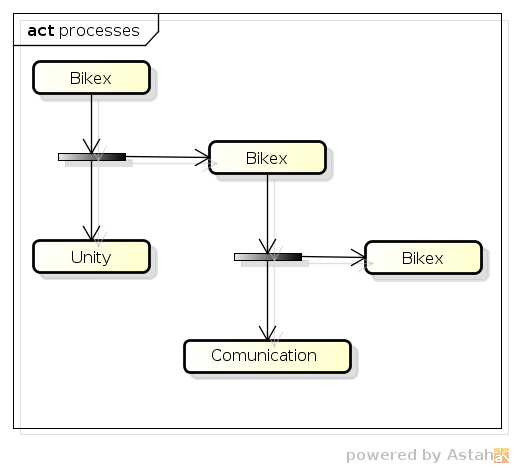
\includegraphics[width=0.6\textwidth]{figuras/processes}
  \caption{Diagrama de Processo}
  \label{fig:diagrama-processo}
\end{figure}

Durante a leitura dos valores dos sensores, é enviado um sinal assíncrono \textbf{SIG1} para o modulo \textit{Comunication}  para requisitar novos valores dos sensores. Após o módulo \textit{Comunication} adquirir os dados enviado pelo módulo \textit{MSP430} pelo método \textit{read\_data}, o dado é escrito em um arquivo pela chamada do método \textit{write\_data} e em fim enviado um sinal assíncrono \textbf{SIG1} para o módulo \textit{Bikex} avisando que os dados já podem ser lidos do arquivo.

\begin{figure}[h]
  \centering
	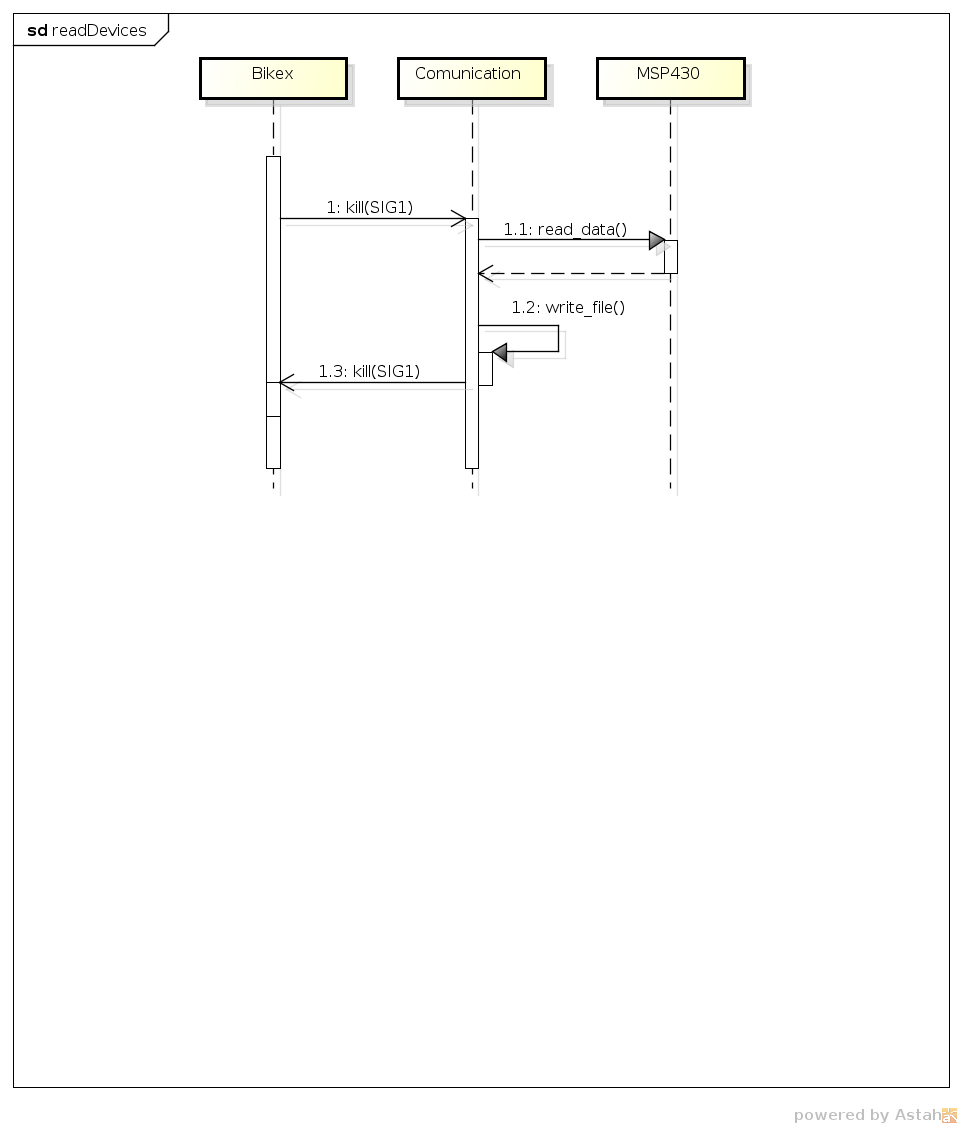
\includegraphics[width=0.7\textwidth]{figuras/readDevices}
  \caption{Diagrama de Sequência para leitura dos sensores passivos}
  \label{fig:diagrama-sequencia-read-devices}
\end{figure}

Feita a leitura dos dados contidos no arquivo, inicia-se a fase de cálculos baseados nestes dados de entrada. Para realizar essa atividade, é enviado um sinal assíncrono \textbf{SIG2} para o módulo \textit{Unity}, que se encarrega em posicionar o objeto corretamente e atualizar a tela atraves do método \textit{render}. O módulo \textit{Unity} retorna então as informações necessárias para que seja atualizado o valor dos sensores ativos do produto atraves de um arquivo  e sinaliza com o sinal assíncrono \textbf{SIG2}.

\begin{figure}[h]
  \centering
	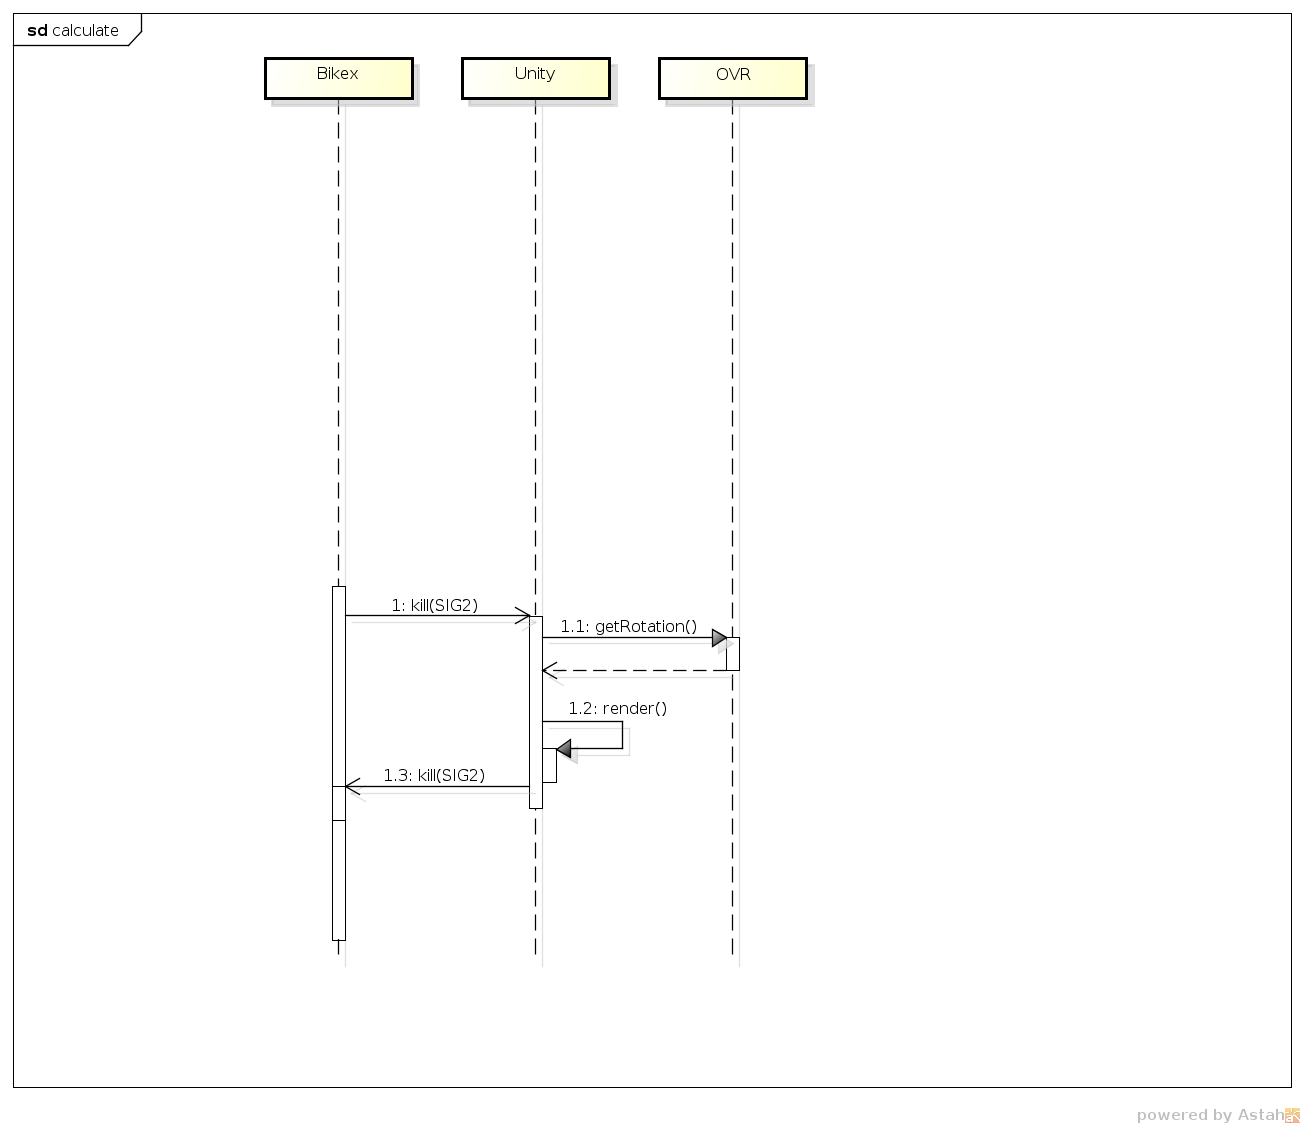
\includegraphics[width=0.7\textwidth]{figuras/calculate}
  \caption{Diagrama de Sequência para processamento de dados e renderização das informações}
  \label{fig:diagrama-sequencia-calculate}
\end{figure}

Para a atualização do estados dos sensores ativos, o Bikex executa o método \textit{writeDevices}, o qual escreve as informações em um arquivo e envia o sinal assíncrono \textbf{SIG3} para o módulo \textit{Comunication}. Por sua vez, o módulo \textit{Comunication} realiza a leitura dos dados no arquivo pelo método \textit{read\_file} e  faz a escrita na porta serial dos valores desejados para os sensores ativos através do método \textit{write\_data}. O MSP430 por sua vez seta os valores recebidos nos sensores ativos.

\begin{figure}[h]
  \centering
	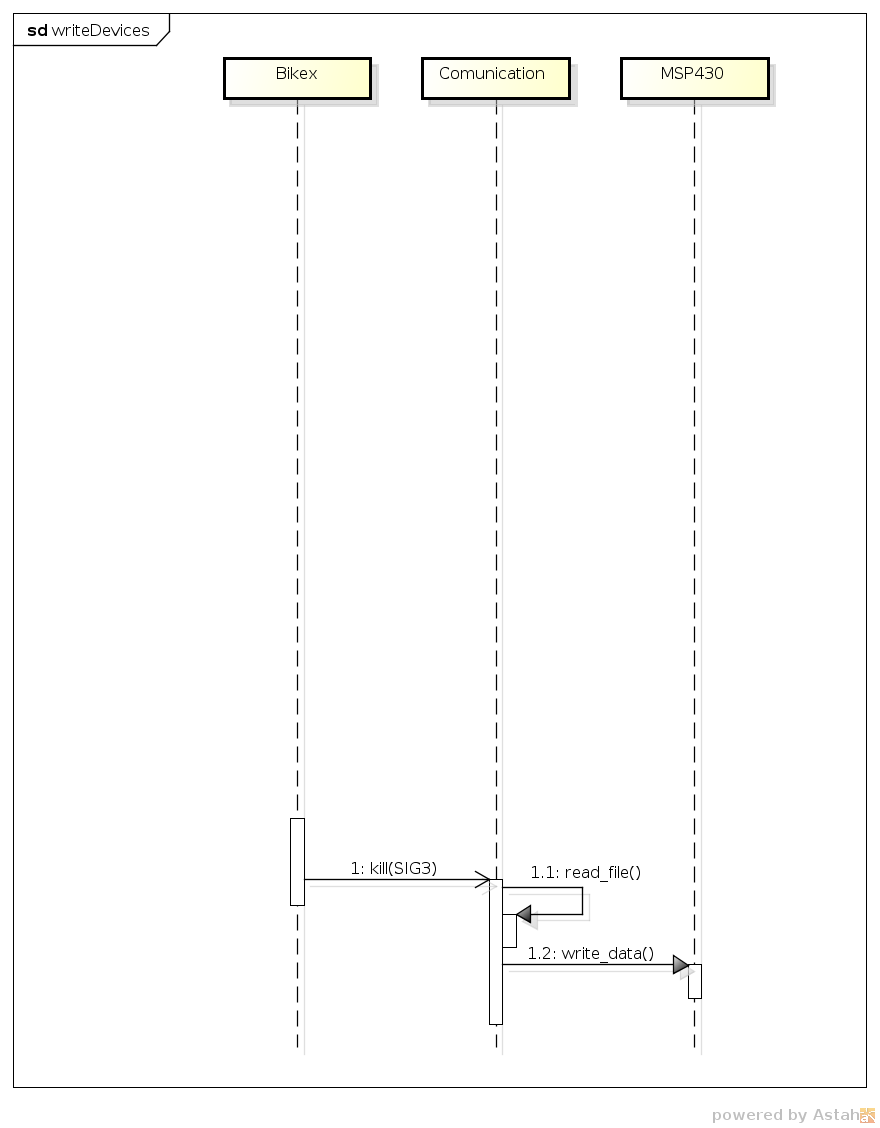
\includegraphics[width=0.7\textwidth]{figuras/writeDevices}
  \caption{Diagrama de Sequência para atualizar valores nos sensores ativos}
  \label{fig:diagrama-sequencia-write-devices}
\end{figure}

%\newpage

\subsection{Diagrama de Classe} % (fold)
\label{sec:diagrama_de_classe}

Para maior compreensão das atividades e responsabilidades de cada classe da aplicação, foi desenhado %o glorioso
diagrama de classes, apresentado na figura \ref{fig:diagrama-classe}.

\begin{figure}[h]
  \centering
	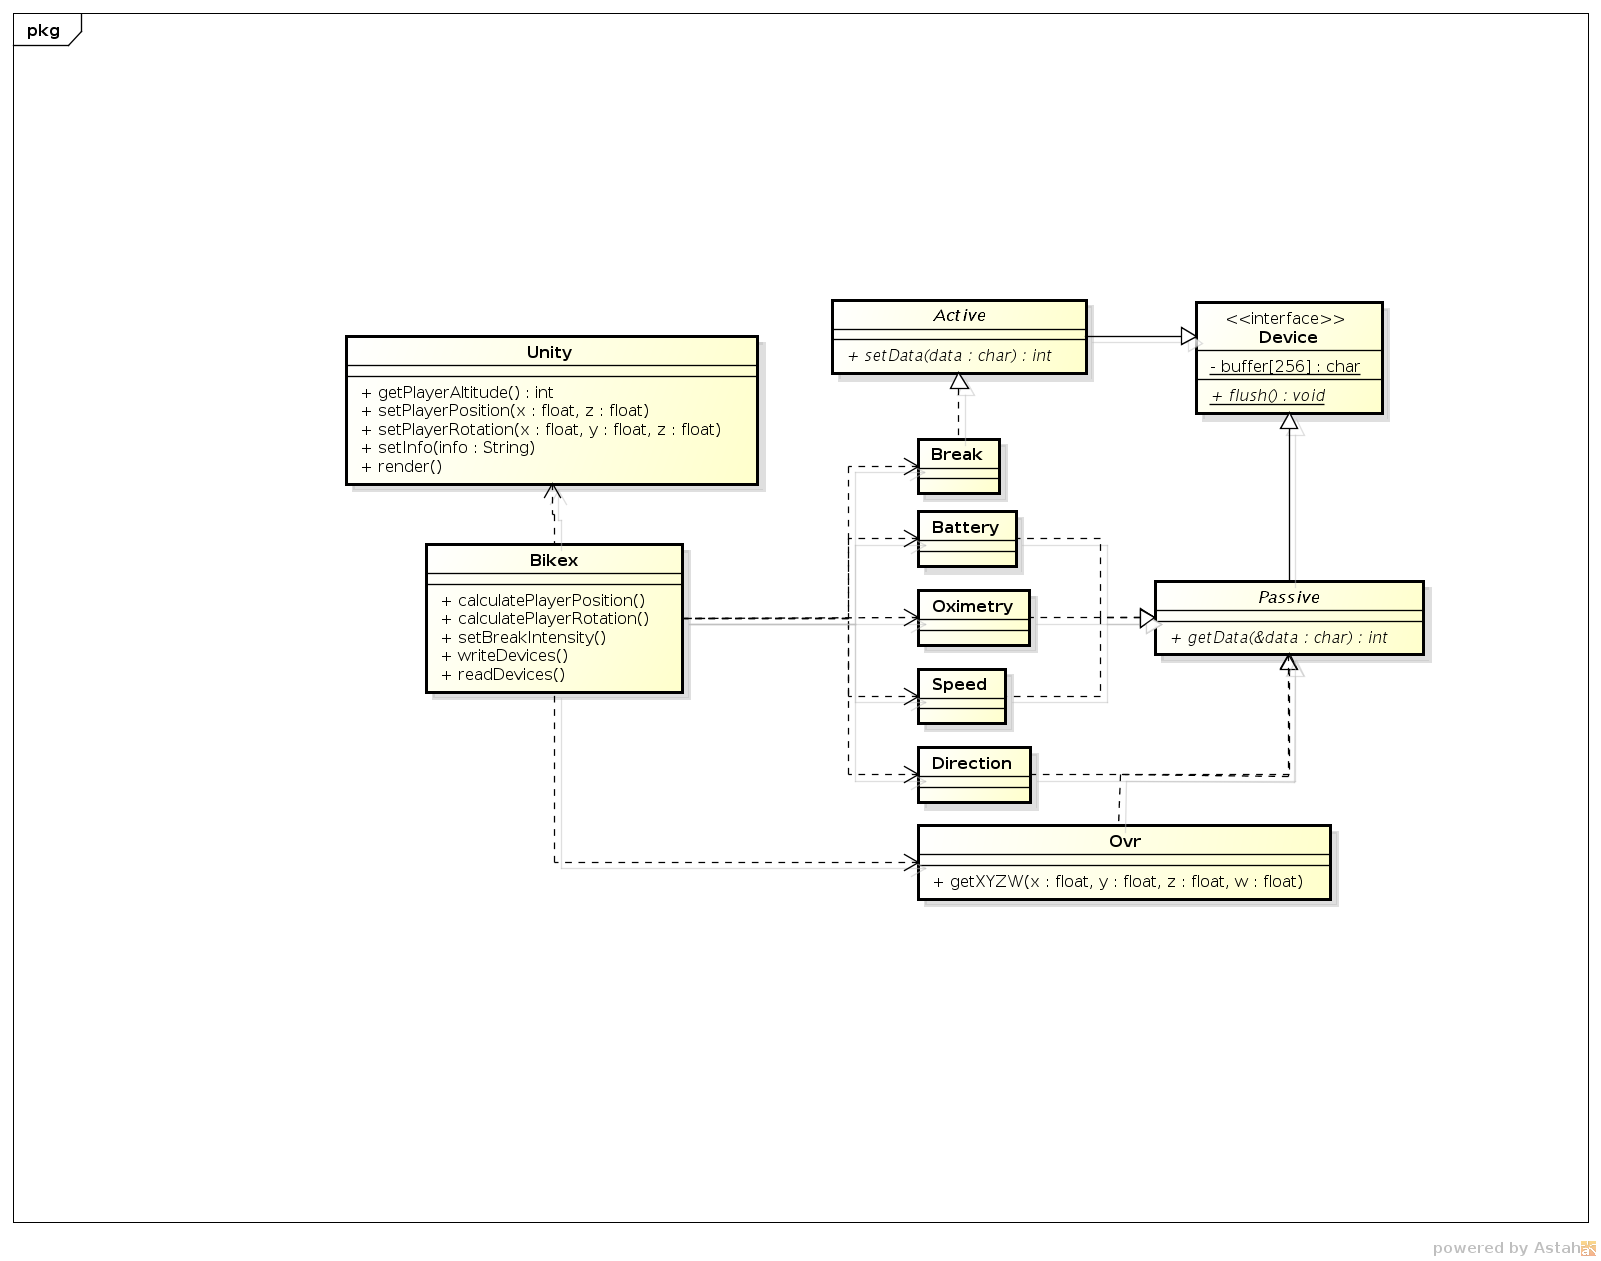
\includegraphics[width=0.8\textwidth]{figuras/class_diagram}
  \caption{Diagrama de Classe}
  \label{fig:diagrama-classe}
\end{figure}

Como o foco do projeto do sistema era a modularidade como um todo, em especial da presença dos sensores, o sistema foi desenhado de forma que seja fácil a adição e remoção de novos sensores, atraves da abstração da interface de comunicação entre os modulo \textit{Bikex} e o \textit{MSP430}.

%\newpage


%Software Bikex: modelagem (uml), linguagem, signals, arquitetura
\subsection{Módulos} \label{sec:modulos}
Esta seção visa descrever como os diversos módulos do sistema irão se comportar separadamente e como vão interagir entre si. O sistema será composto pelos Unity, Bikex, Device.

O módulo Unity será responsável com as interações entre o usuário e o sistema. A primeira responsabilidade é retornar para o sistema a altitude atual do usuário. Essa informação será usada para definir se é necessário o acionamento da frenagem para simular uma inclinação no ambiente virtual. Outra responsabilidade será definir a posição e rotação atual do usuário no sistema. Essas informações irão ser disponibilizadas com a interação de outros módulos. Algumas informações serão disponibilizadas pelo sistema para o usuário. Informações como: velocidade, distância e a velocidade máxima atingida pelo usuário. Por fim, esse módulo irá fazer a renderização do frame para o usuário. Essa renderização irá considerar todas as interações com o sistema e as informações geradas com essa interação.

No sistema terá um módulo que será composto por várias classes. Esse módulo, que é o responsável em fazer a interação com os dispositivos externos, se chama Device. Primeiramente, a classe principal será uma interface chamada Device. Duas classes irão relacionar com essa interface diretamente, a Active e a Passive. A classe Active representará os dispositivos que irão influenciar ativamente e fisicamente no sistema. Essa classe irá ser responsável por informar os dados para essa influência no sistema. Um dispositivo que exemplificar é a frenagem do sistema. A classe Passive são dispositivos que fornecem informações para o sistema. Os dispositivos de velocidade, direção e OVR são exemplos desse tipo de Device. A classe Passive irá ser responsável de coletar informações desses dispositivos e fornecer para o sistema realizar os procedimentos necessários. O dispositivo OVR é o Oculus em si e será responsável em fornecer a posição da cabeça do usuário.

O módulo Bikex é o módulo central do sistema e fará a interface com o módulo Unity e os outros módulos. Esse módulo é responsável por receber as informações dos dispositivos do tipo Passive e fazendo as transformações necessárias para enviar para o módulo Unity. O primeiro procedimento que esse módulo realiza é o cálculo da posição do usuário e tem como entrada a velocidade e a direção atuais do usuário. Outro procedimento será o cálculo da rotação do usuário. Isso será feito a partir de dados fornecidos pelo dispositivo Oculus. Essa rotação definirá a direção que o usuário está olhando. Definimos a separação desses dois procedimentos para que a rotação da cabeça do usuário não interfira na rotação da bicicleta. O outro procedimento é definir a intensidade de frenagem de acordo com a altitude coletada do módulo Unity. A partir dessa intensidade, o Bikex aciona o dispositivo de freio com a mesma.



%Unity: scripts, modelagem, assets etc
\subsection{Unity}

%Python: versao do python, modulos puppet, modulos para comunicacao UART
\subsection{Interface Python} % (fold)
\label{sec:interface_python}

A interface \gls{python} sim1plifica a comunicação com o microcontrolador, possibilitando o \textit{parse} entre o modulo principal (BikeX \ref{sec:sistema_bikex}) e o \gls{msp}.

A interface faz de uso da biblioteca \href{http://pyserial.sourceforge.net/pyserial.html}{Pyserial} para manter a comunicação com o microcontrolador. Devido as inúmeras possibilidades de conflitos existentes de caracteres e velocidade de comunicação existentes na comunicação \gls{rs232}, os desenvolvedores da \textit{Pyserial} construíram a classe \textit{serial.tools.miniterm} na qual simula um terminal de comunicação como exemplo de uso da biblioteca. O grupo construiu então uma classe que herda da \textit{serial.tools.miniterm}, simplificando assim a comunicação e incrementando a estabilidade de comunicação. Esta ação gera a dependência de que a versão da \textit{Pyserial} necessita ser 2.7 ou superior.

\subsubsection{Visão do BikeX} % (fold)
\label{sub:vis_o_do_bikex}

Do ponto de vista do BikeX a aplicação Python estará rodando sempre em \textit{background} esperando um sinal para a realização de alguma tarefa. A depender do sinal recebido, será realizado uma leitura do estado dos sensores ou o envio do valor de posicionamento do freio.

% Por ser um programa assíncrono, a aplicação passará grande parte do tempo ociosa.
A tomada de uso de sinais para acordar o processo possibilita que o mesmo se mantenha em descanso durante todo o período em que não há requisição de dados. Como resultado do ponto de vista da arquitetura que suportado software, não há uma sobrecarga de processamento, evitando o \textit{overhead} de requisições desnecessárias e possibilitando assim que o processamento possa ficar focado onde realmente há uma grande demanda de CPU e GPU, que é a interface gráfica da aplicação.

No trecho de código a seguir (\ref{trecho_main_py}) é possível observar a rotina principal da aplicação \textit{Python} populando o objeto do MSP430 com alguns dispositivos e definindo os métodos a serem chamados na ocorrência dos sinais já pré-definidos. Em seguida o programa entra no já referido \textit{loop}, permanecendo nele ate receber um sinal que requisite o termino do processo.

\begin{lstlisting}[language=Python,caption={Trecho da rotina principal do script Python},label=trecho_main_py]
def main():
    pid_bikex = sys.argv[1:2]
    msp430.curb = sensor.Break(msp430.serial,0)
    msp430.velocity = sensor.Velocity(msp430.serial,0)
    msp430.passives = sensor.Passives(msp430.serial,0)


    signal(SIG1, write_file)
    signal(SIG3, read_file)
    signal(SIGINT, safe_quit)
    signal(SIGQUIT, safe_quit)
    signal(SIGABRT, safe_quit)
    while True:
        sleep(0.01)

\end{lstlisting}


\subsubsection{Visão do MSP430} % (fold)
\label{sub:vis_o_do_msp430}

Do ponto de vista do MSP430 a aplicação Python estará sempre em comunicação ativa com o MSP430, já que a porta serial será aberta assim que o sistema for iniciado e só fechará quando programa vier a fechar.

Como apresentado no código \ref{trecho_main_py}, a aplicação Python estará sempre a espera de um sinal para entrar em contato com o MSP430. Para que ocorra a interação, é enviado um comando especifico ao MSP430 sobre qual dispositivo desejamos ter informação. No código \ref{trecho_device_py} podemos observar a declaração de algumas classes de dispositivos passivos na estrutura física do projeto, como o freio. Todos os dispositivos herdam de uma classe primaria que tem declarada uma sequencia básica de leitura-escrita de comandos no MSP430.


\begin{lstlisting}[language=Python,caption={Declaração de classes fundamentais no script Python},label=trecho_device_py]
class Passive(Device):
    """docstring for Active"""
    def __init__(self, terminal):
        super(Passive, self).__init__(terminal)
        self.data = self.serial.readline()
        self.data = self.data.split('\n')[0]

    def read_data(self, command):
        """ Send some data to device """
        self.serial.write(str(command))
        self.data = self.serial.readline()
        self.data = self.data.split('\n')[0]
        return self.data

    def write_data(self, command, data):
        return None

class Velocity(Passive):
    """docstring for Velocity"""
    def __init__(self,terminal, arg=VELOCITY_MSP):
        super(Velocity, self).__init__(terminal)
        self.arg = arg
        
    def read_data(self):
        return super(Velocity, self).read_data(self.arg)

class Passives(Passive):
    """docstring for Passives"""
    def __init__(self,terminal, arg=ALL_VALUES):
        super(Passives, self).__init__(terminal)
        self.arg = arg
        
    def read_data(self):
        return super(Passives, self).read_data(self.arg)
\end{lstlisting}

Definido uma interface padrão de leitura-escrita nos dispositivos, é então instanciado no objeto \textbf{MSP} a os dispositivos desejados para que a rotina principal possa interagir com os dispositivos. Para uma mair comodidade e melhor visualização da escrita do código, foram definidos os métodos \textit{\_\_getitem\_\_} e \textit{\_\_setitem\_\_} da classe \textbf{MSP}, conforme apresentado a seguir:

\begin{lstlisting}[language=Python,caption={Declaração dos métodos de leitura e escrita de item},label=trecho_item_py]
    def __getitem__(self,key):
        """ Return the value of a item """
        try:
            return getattr(self,key).read_data()
        except Exception, e:
            raise e

    def __setitem__(self,key,item):
        """ Set a value of a item """
        getattr(self,key).write_data(str(item))
\end{lstlisting}

As rotinas implementadas no trecho do código \ref{trecho_item_py} permitem a leitura e o envio de algum valor, respectivamente, de um possível atributo \textit{foo} - meramente ilustrativo de exemplo - da seguinte forma:

\begin{lstlisting}[frame=none,numbers=none]  % Start your code-block

>>> msp430.foo = sensor.Passives(msp430.serial,0)
>>> print msp430['foo']
>>> 33
>>> """Sending some value"""
>>> msp430['foo'] = 30
\end{lstlisting}

Obviamente que, como visto no código \ref{trecho_device_py}, o método de escrita de objetos passivos se resume a retornar um objeto nulo, não interagindo assim com o MSP430. Porém, esta solução permite que, se houvesse o interesse em fazer de uso de algum dispositivo no MSP430 que pudesse assumir estados e retornar valores, a interação com ele seria a mais transparente possível. Um possível exemplo seria uma segunda porta de comunicação, seja ela UART ou algum outro protocolo de comunicação como $CAN$ ou $I^2C$. Da mesma forma que poderíamos enviar uma \textit{string} pela UART para ser equalizada na outra porta, poderíamos receber uma mensagem nova pela mesma.

% Os códigos na integra podem ser observados nas sessões \ref{main_py}, \ref{device_py} e \ref{msp430_py}  nos anexos.


%Falar aqui sobre o software do bikex, a integracao do python/msp430/unity
\subsection{Integração Sensores e Sistema}
